\documentclass[12pt]{article}

\usepackage[dutch]{babel}
\usepackage{a4wide}
\usepackage{amsmath}
\usepackage{enumerate}
\usepackage{eurosym}
\usepackage{url}
\usepackage{graphicx}

\author{Jos Bonsink \& Mustafa Karaalioglu}

\begin{document}

\title{Project verslag - Project Thunder}
\maketitle

\section{Abstract}

\section{Inleiding}

\section{Materiaal en methode}
De experimenten met de Android-applicatie werden uitgevoerd op HTC Desire C telefoons met Android 4.0.2. Om positiebepaling mogelijk te maken met deze telefoons moesten er drie problemen worden opgelost: Bluetooth communicatie, audio detectie en afstandsmeting.

\subsection{Audio detectie}
Voor het realtime detecteren van piepgeluiden moest er constant geluid opgenomen \'en geanalyseerd worden.
De audiohardware bufferde continu een halve seconde aan audio. In een aparte thread werden er steeds twintig samples uit deze buffer opgehaald. Op deze samples werd een Fast Fourier Transformatie(FFT) toegepast. Hiermee werd het geluidssignaal als functie van tijd omgezet naar een complexe functie van amplitude en fase als functie van frequentie. 

De gegenereerde piepgeluiden bestonden uit een sinuso\"ide met een frequentie van $8820$ Hz. Na de FFT werd de lengte van het complexe getal corresponderend met de frequentie van het piepgeluid vergeleken met een drempelwaarde. Wanneer de lengte de drempelwaarde overschreed, werd het geluid herkend als een piep.

\subsection{Afstandsmeting}
De afstand tussen twee Android-apparaten werd bepaald door het tijdsverschil tussen het verzenden en ontvangen van gegenereerde piepgeluiden te meten. Uit de eerder genoemde lijst van mac-adressen in het Bluetooth-netwerk werden een \textit{master} en \textit{slave} uitgekozen aan de hand van de volgorde van de lijst. De master verzocht via Bluetooth de slave te antwoorden op zijn piepgeluid. Na bevestiging van de slave, speelde de master een piepgeluid af.

Het tijdsverschil tussen het versturen en ontvangen van piepgeluiden kon worden gemeten door het aantal samples tussen twee piepgeluiden te gebruiken. Het twee keer achterelkaar detecteren van hetzelfde piepgeluid, werd voorkomen door een korte periode na een detectie niks te detecteren. De looptijd kon exact worden verkregen door te corrigeren voor de verwerkingstijd die nodig is bij het afspelen van geluid. Voor de master werd het aantal samples tussen de detectie van zijn eigen piep en dat van de respons gemeten. Bij de slave werd het verschil gemeten tussen de detectie van het eerste piepgeluid en dat van zichzelf. Dit verschil werd via Bluetooth naar de master verstuurd. De master trok deze waarde af van de gemeten totaal aantal samples totdat een andere piep werd gehoord. Aan de hand van de samplerate (44100Hz) kon de tijdsduur worden bepaald, hiermee kon vervolgens de afstand worden berekend.

\section{Resultaten}
\begin{figure}[h]
\centering
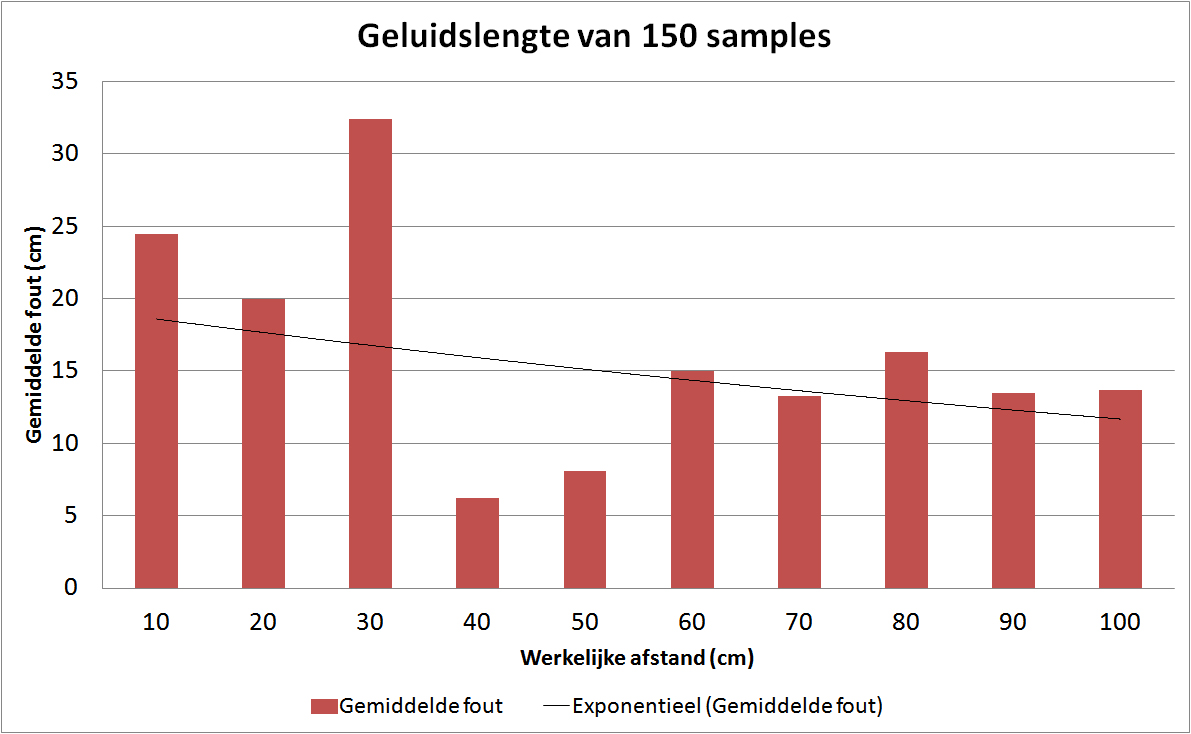
\includegraphics[scale=0.4]{150-samples}
\caption{Gemiddelde fout bij piepgeluid met geluidslengte van 150 samples.}
\end{figure}

\begin{figure}[h]
\centering
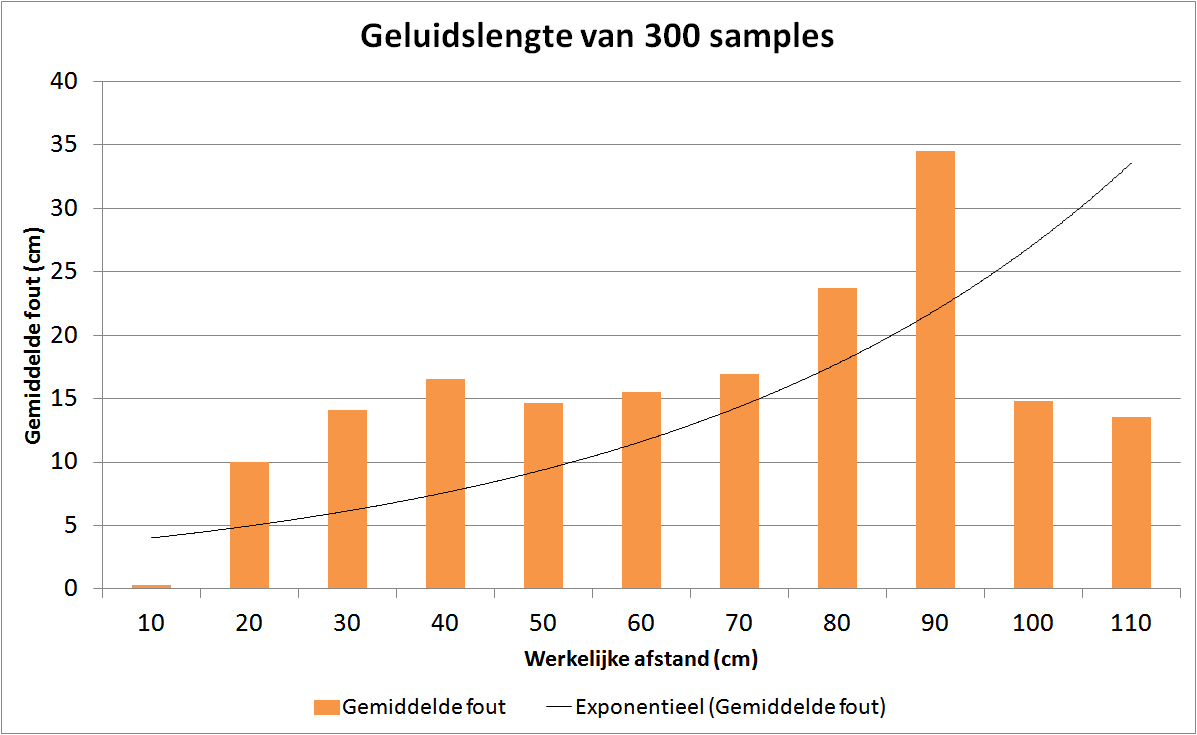
\includegraphics[scale=0.4]{300-samples}
\caption{Gemiddelde fout bij piepgeluid met geluidslengte van 150 samples.}
\end{figure}

\section{Discussie}

\section{Nawoord}

\end{document}



